% begin module arc-length-ex1
\begin{frame}
\begin{example} 
Find the length of the arc of $y^2 = x^3$ between $(1,1)$ and $(4,8)$.
\begin{columns}[c]
\column{.3\textwidth}
%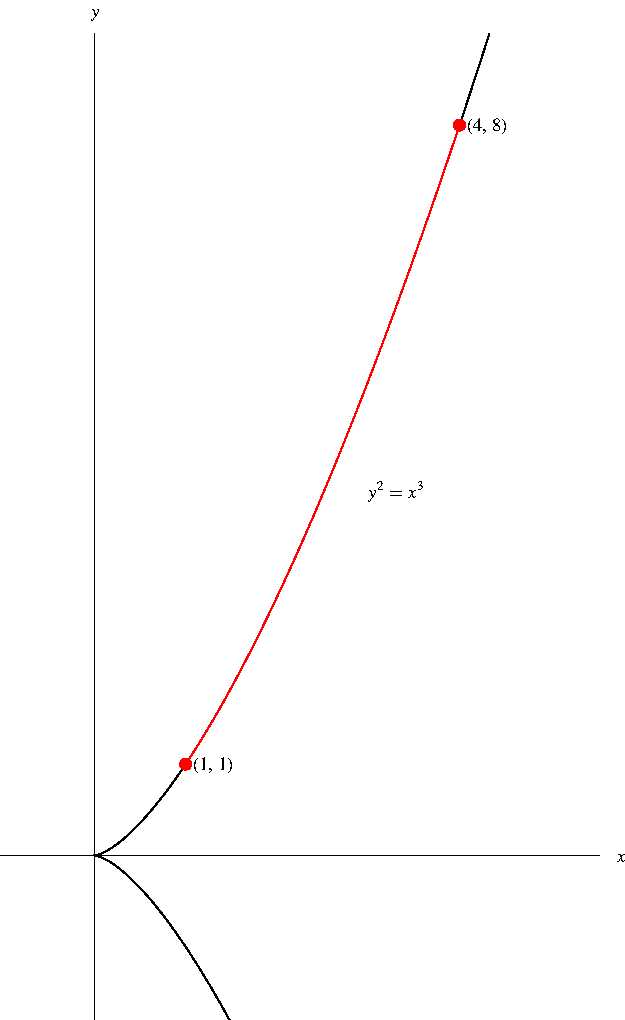
\includegraphics[height=6cm]{arc-length/pictures/09-01-ex1.pdf}%
\psset{xunit=0.4cm, yunit=0.4cm}
\begin{pspicture}(-0.9, -8.955949)(6,9.055949)
\tiny
\fcAxesStandard{-0.65}{-8.705949}{5.5}{8.705949}
%Function formula: - \sqrt{x^{3}}
\psplot[linecolor=gray, plotpoints=1000]{0}{4.2}{x 3 exp sqrt -1 mul }
%Function formula: \sqrt{x^{3}}
\psplot[linecolor=gray, plotpoints=1000]{0}{4.2}{x 3 exp sqrt }
%Function formula: \sqrt{x^{3}}
\psplot[linecolor=\fcColorGraph, plotpoints=1000]{1}{4}{x 3 exp sqrt }
\fcFullDot{1}{1}
\fcFullDot{4}{8}
\rput[tl](4.2, 8){$(4,8)$}
\rput[tl](1.2, 1){$(1,1)$}
\rput[l](2.7, 4){$y^2=x^3$}
\end{pspicture}
\column{.7\textwidth}
\begin{itemize}
\item<2->  For the top half of the curve we have:
\item<2->  \alertNoH{ 3-4}{$y = \uncover<4->{x^{3/2}}$} and  \alertNoH{ 5-6,8}{$y' = \uncover<6->{\frac{3}{2}x^{1/2}}$}.
\item<9->  \alertNoH{ 10-11}{$u = \uncover<11->{1 + \frac{9}{4}x}$} and  \alertNoH{ 12-13}{$\diff u = \uncover<13->{\frac{9}{4}\diff x}$}.
\item<9-| alert@14-15>  When $x = 1$, $u = \uncover<15->{\frac{13}{4}}$.
\item<9-| alert@16-17>  When $x = 4$, $u = \uncover<17->{10}$.
\end{itemize}
\begin{eqnarray*}
\uncover<7->{%
L %
}%
& \uncover<7->{ = } &%
\uncover<7->{%
\int_1^4 \sqrt{1+\left( \alertNoH{ 8}{y'} \right)^2}\diff x%
}\\%
& \uncover<8->{ = } &%
\uncover<8->{%
\int_{\alertNoH{ 14-15}{1}}^{\alertNoH{ 16-17}{4}} \sqrt{\alertNoH{ 11}{1+} \alertNoH{ 8,11}{\frac{9}{4}x} }\ \alertNoH{ 12-13}{\diff x}%
} \uncover<9->{ = } \uncover<9->{%
\int_{\alertNoH{ 14-15}{\uncover<15->{13/4}}}^{\alertNoH{ 16-17}{\uncover<17->{10}}} \alertNoH{ 12-13}{\uncover<13->{\frac{4}{9}}}\uncover<11->{\sqrt{\alertNoH{ 10-11}{u}}}\ \alertNoH{ 12-13}{\uncover<13->{\diff u}}%
}\\%
& \uncover<18->{ = } &%
\uncover<18->{%
\frac{4}{9}\left[ \frac{2}{3} u^{3/2}\right]_{13/4}^{10}%
} \uncover<19->{ = } \uncover<19->{%
\frac{8}{27}\left( 10^{3/2} - \left( \frac{13}{4}\right)^{3/2}\right)%
}\\%
\end{eqnarray*}
\end{columns}
\end{example}
\end{frame}
% end module arc-length-ex1
